\input{"../../../preamble"}

\begin{document}

\title{CSC263-Notes-01-28-2015}

\input{"../csc263-header"}
\rhead{January 28, 2015}

\section*{Lecture 08}

\begin{center}
\begin{tabular}{c c c}

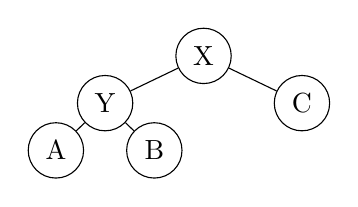
\begin{tikzpicture}[every node/.style={circle,draw,minimum size=2em,inner sep=1},
	baseline={(current bounding box.center)},
	level/.style={level distance=6mm,
	sibling distance=25mm/#1}]
\node {X} 
child {node {Y}
	child {node {A}}
	child {node {B}}
	}
child {node {C}};
\end{tikzpicture} &

\pbox{10cm}{
	rotate right $\rightarrow$ \\
	$\leftarrow$ rotate left
} & 

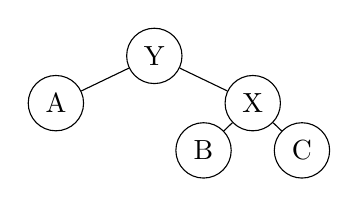
\begin{tikzpicture}[every node/.style={circle,draw,minimum size=2em,inner sep=1},
	baseline={(current bounding box.center)},
	level/.style={level distance=6mm,
	sibling distance=25mm/#1}]
\node {Y} 
child {node {A}}
child {node {X}
	child { node{B}}
	child { node{C}}
	};
\end{tikzpicture}
\end{tabular}
\end{center}
\begin{lstlisting}[language=Python,mathescape]
AVL-insert(root, x):
	if root == NIL: # found insertion point
		root = TreeNode(x) # initial height = 0
	else if x.key < root.item.key:
		root.left = AVL-insert(root.left, x)
		if root.left.height > root.right.height + 1:
			root = AVL-rebalance-right(root)
		else: # no rebalancing, but height might have changed
			AVL-update-height(root)
	else if x.key > root.item.key:
		root.right = AVL-insert(root.right, x)
		if root.right.height > root.left.height + 1:
			root = AVL-rebalance-to-the-left(root)
		else: 
			AVL-update-height(root)
	else: # x.key = root.item.key
		root.item = x
	return root
\end{lstlisting}

\begin{lstlisting}[language=Python,mathescape]
AVL-rebalance-to-the-left(root):
	if root.right.left.height > root.right.right.height:
		root.right = AVL-rotate-to-the-right(root.right)
	return AVL-rotate-to-the-left(root)

AVL-rebalance-to-the-right(root):
	if root.left.right.height > root.left.left.height:
		root.left = AVL-rotate-to-the-left(root.left)
	return AVL-rotate-to-the-right(root)

AVL-rotate-to-the-left(y):
	x = y.right
	y.right = x.left
	x.left = y
	AVL-update-height(x.left);
	AVL-update-height(x);
	return x

AVL-rotate-to-the-right(y):
	x = y.left
	y.left = x.right
	x.right = y
	AVL-update-height(x.right)
	AVL-update-height(x)
	return x
	
AVL-update-height(node):
	node.height = 1 + max(node.left.height, node.right.height)
\end{lstlisting}

\noindent No checking for special cases when references are \texttt{NIL} $\ldots$
\textbf{Trick} $\rightarrow$ Define NIL node: \\
\indent NIL.item = NIL \\
\indent NIL.left = NIL \\
\indent NIL.right = NIL \\
\indent NIL.height = -1 \\
Use just one \texttt{NIL} node for the entire tree: every node with a reference to \texttt{NIL} refers to the same \texttt{NIL}. Now, no need for lots of extra code to check for \texttt{NIL} before each access!

\subsection*{\texttt{delete}}

\noindent Like \texttt{delete} on BST. After every recursive call:
\begin{enumerate}[label={(\arabic*)}]
	\item check if subtrees have become unbalanced
	\item rebalance with rotations
	\item update heights
\end{enumerate}

\begin{lstlisting}[language=Python,mathescape]
AVL-remove(root, x):
	if root == NIL:
		pass
	else if x.key < root.item.key:
		root.left = AVL-remove(root.left, x)
		if root.right.height > root.left.height + 1:
			root = AVL-rotate-to-the-left(root)
		else:
			AVL-update-height(root)
	else if x.key > root.item.key:
		root.right = AVL-remove(root.right, x)
		if root.left.height > root.right.height + 1:
			root = AVL-rebalance-to-the-right(root)
		else:
			AVL-update-height(root)
	else:
		if root.left == NIL or root.right == NIL:
			if root.left == NIL:
				root = root.right
			else:
				root = root.left
		else:
			# Select whether to replace root.item with its predecessor or
			# its successor, depending on the heights of subtrees
			if root.left.height > root.right.height:
				root.item, root.left = AVL-remove-max(root.left)
			else:
				root.item, root.right = AVL-remove-min(root.right)
			AVL-update-height(root)
	return root

AVL-remove-min(root):
	if root.left == NIL:
		return root.item, root.right
	else:
		item, root.left = tree-remove-min(root.left)
		AVL-update-height(root)
		return item, root

AVL-remove-max(root):
	if root.right == NIL:
		return root.item, root.left
	else:
		item, root.right = tree-remove-max(root.right)
		AVL-update-height(root)
		return item, root
\end{lstlisting}

\subsubsection*{\texttt{search}}

\noindent Unchanged.

\begin{lstlisting}[language=Python]
AVL-search(root, k):
	if root == NIL:
		pass
	else if k < root.item.key:
		root = AVL-search(root.left, k)
	else if k > root.item.key:
		root = AVL-search(root.right, k)
	else:
		pass
	return root
\end{lstlisting}


\subsection*{Augmented Data Structures}

\noindent Existing data structure modified to store additional information and/or perform additional operations.\\
In general:
\begin{enumerate}[label={(\arabic*)}]
	\item Choose data structure to augment
	\item Determine additional info
	\item Check additional info can be maintained in every old operation. (and at what additional cost?)
	\item Implement new operations
\end{enumerate}

\subsection*{Ordered Sets}

\noindent set = $\{144, 20, 100, 40, 17\}$\\
Operations \texttt{insert}, \texttt{delete}, \texttt{search}\\
\texttt{rank(k)} - index of $k$ in a sorted ordering of set elements [17,20,40,100,144] \\
\texttt{select(rank)} $\rightarrow$ 

\end{document}
